\documentclass{article}

% content/resources/templates/preamble.tex
\usepackage[margin=0.6in]{geometry}
\author{Milav Dabgar}
\usepackage{amsmath,amssymb,amsthm}
\usepackage{booktabs}
\usepackage{multirow}
\usepackage{xcolor}
\usepackage{tcolorbox}
\tcbuselibrary{breakable,skins}
\usepackage[colorlinks=true,linkcolor=blue]{hyperref}
\usepackage{titlesec}
\usepackage{enumitem}
\usepackage{tikz}
\usepackage{pgfplots}
\usepackage{circuitikz}
\usepackage[version=4]{mhchem}
\usepackage{longtable}
\usepackage{array}
\usepackage{float}
\usepackage{caption}
\usepackage{listings}

\lstset{
  basicstyle=\small\ttfamily,
  breaklines=true,
  breakatwhitespace=false,
  postbreak=\mbox{\textcolor{red}{$\hookrightarrow$}\space},
  float=false,
  numbers=left,
  numberstyle=\tiny\color{gray},
  numbersep=10pt,
  xleftmargin=2em,
  keywordstyle=\color{blue},
  commentstyle=\color{green!60!black},
  stringstyle=\color{purple},
  backgroundcolor=\color{gray!5},
  showstringspaces=false,
  tabsize=2,
  captionpos=b,
  keepspaces=true,
  columns=flexible
}

\pgfplotsset{compat=1.18}
\usetikzlibrary{shapes,arrows,positioning,calc,patterns,decorations.pathmorphing,decorations.markings,arrows.meta}

% Color scheme
\definecolor{headcolor}{RGB}{0,102,204}
\definecolor{keycolor}{RGB}{220,20,60}
\definecolor{solutioncolor}{RGB}{34,139,34}
\definecolor{mnemoniccolor}{RGB}{148,0,211}
\definecolor{codecolor}{RGB}{0,0,100}

% Spacing
\setlength{\parskip}{3pt}
\setlist[itemize]{nosep}
\setlist[enumerate]{nosep}

% Title formatting
\titleformat{\section}{\Large\bfseries\color{headcolor}}{\thesection}{1em}{}
\titleformat{\subsection}{\large\bfseries\color{headcolor}}{\thesubsection}{1em}{}

% Pandoc tightlist compatibility
\providecommand{\tightlist}{%
  \setlength{\itemsep}{0pt}\setlength{\parskip}{0pt}}

% Pandoc longtable compatibility
\newcounter{none}
\def\thenone{}


% content/resources/templates/english-boxes.tex

% Custom environments
\newtcolorbox{solutionbox}{
 breakable,
 enhanced,
 colback=solutioncolor!5!white,
 colframe=solutioncolor!75!black,
 fonttitle=\bfseries,
 title=Solution
}

\newtcolorbox{solutionboxnobreak}{
 colback=solutioncolor!5!white,
 colframe=solutioncolor!75!black,
 fonttitle=\bfseries,
 title=Solution
}

\newtcolorbox{keyformula}{
 breakable,
 enhanced,
 colback=keycolor!5!white,
 colframe=keycolor!75!black,
 fonttitle=\bfseries,
 title=Key Formula
}

\newtcolorbox{mnemonicboxenv}{
 breakable,
 enhanced,
 colback=mnemoniccolor!5!white,
 colframe=mnemoniccolor!75!black,
 fonttitle=\bfseries,
 title=Mnemonic
}

\newcommand{\mnemonicbox}[1]{%
  \begin{mnemonicboxenv}
    #1
  \end{mnemonicboxenv}
}


% Custom commands for GTU solutions
% This file defines semantic commands for consistent formatting

% Question command with automatic formatting
\newcommand{\question}[2]{%
  \section*{Question #1}%
  \textbf{#2}%
}

% OR question variant
\newcommand{\questionor}[2]{%
  \section*{Question #1 OR}%
  \textbf{#2}%
}

% Proper table environment with caption
\newenvironment{answertable}[1]{%
  \begin{table}[htbp]
  \centering
  \caption{#1}
}{%
  \end{table}
}

% Proper figure environment for diagrams
\newenvironment{answerdiagram}[1]{%
  \begin{figure}[htbp]
  \centering
  \caption{#1}
}{%
  \end{figure}
}

% Semantic markup for key terms
\newcommand{\keyword}[1]{\textbf{#1}}
\newcommand{\code}[1]{\texttt{#1}}
\newcommand{\classname}[1]{\texttt{#1}}
\newcommand{\methodname}[1]{\texttt{#1}}

% Proper quotation marks
\newcommand{\mnemonic}[1]{``#1''}


\title{Physics (4300005) - Winter 2023 Solution}
\date{January 16, 2024}

\begin{document}
\maketitle

\questionmarks{1(a)}{3}{Define: (a) Meter (b) Kelvin (c) Accuracy.}

\begin{solutionbox}
\begin{itemize}
    \item \textbf{Meter}: The meter is the SI unit of length, defined as the distance traveled by light in vacuum during a time interval of 1/299,792,458 of a second.
    \item \textbf{Kelvin}: The kelvin is the SI unit of thermodynamic temperature, defined by setting the fixed numerical value of the Boltzmann constant k to $1.380649 \times 10^{-23}$ J/K.
    \item \textbf{Accuracy}: Accuracy is the degree of closeness of a measured value to the true or standard value of the quantity being measured.
\end{itemize}
\end{solutionbox}

\begin{mnemonicbox}
\mnemonic{MKA - Meter measures Kilometers Accurately}
\end{mnemonicbox}

\questionmarks{1(b)}{4}{Explain construction of Vernier calipers with clean figure.}

\begin{solutionbox}
\textbf{Diagram:}
\begin{center}
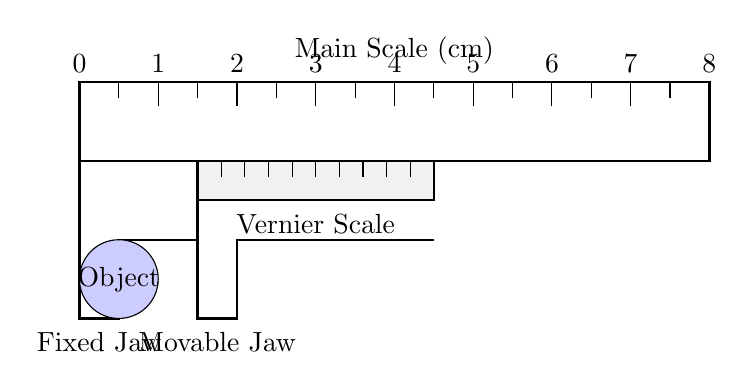
\begin{tikzpicture}
    % Main Scale
    \draw[thick] (0,0) rectangle (8,1);
    \foreach \x in {0,1,...,8} \draw (\x,1) -- (\x,0.7) node[above=3mm] {\x};
    \foreach \x in {0.5,1.5,...,7.5} \draw (\x,1) -- (\x,0.8);
    \node at (4,1.4) {Main Scale (cm)};
    
    % Vernier Scale
    \draw[thick, fill=gray!10] (1.5,-0.5) rectangle (4.5,0);
    \foreach \x in {1.5,1.8,...,4.5} \draw (\x,0) -- (\x,-0.2);
    \node at (3,-0.8) {Vernier Scale};
    
    % Jaws
    \draw[thick] (0,0) -- (0,-2) -- (0.5,-2) -- (0.5,-1) -- (1.5,-1) -- (1.5,0);
    \node at (0.25,-2.3) {Fixed Jaw};
    
    \draw[thick] (1.5,-0.5) -- (1.5,-2) -- (2,-2) -- (2,-1) -- (4.5,-1);
    \node at (1.75,-2.3) {Movable Jaw};
    
    % Object
    \draw[fill=blue!20] (0.5,-1.5) circle (0.5);
    \node at (0.5,-1.5) {Object};
\end{tikzpicture}
\captionof{figure}{Vernier Calipers Construction}
\end{center}

Vernier calipers consist of:
\begin{itemize}
    \item \textbf{Main scale}: Fixed scale marked in standard units (mm or inches)
    \item \textbf{Vernier scale}: Movable scale that slides along the main scale
    \item \textbf{Fixed jaw}: Attached to the main scale
    \item \textbf{Movable jaw}: Connected to the vernier scale
    \item \textbf{Depth probe}: For measuring depth of cavities
    \item \textbf{External jaws}: For measuring outer dimensions
    \item \textbf{Internal jaws}: For measuring inner dimensions
\end{itemize}
\end{solutionbox}

\begin{mnemonicbox}
\mnemonic{FMMVJ - Fixed Main scale Makes Vernier Jaw move}
\end{mnemonicbox}

\questionmarks{1(c)(1)}{4}{What is physical quantities? Explain its types depending on direction.}

\begin{solutionbox}
A physical quantity is a measurable property of a physical system that can be quantified by measurement.

\textbf{Types of physical quantities based on direction:}

\begin{center}
\captionof{table}{Scalar vs Vector Quantities}
\begin{tabulary}{\linewidth}{|L|L|}
\hline
\textbf{Scalar Quantities} & \textbf{Vector Quantities} \\ \hline
Have only magnitude & Have both magnitude and direction \\ \hline
Examples: mass, time, temperature, energy & Examples: displacement, velocity, force, acceleration \\ \hline
Represented by simple numbers & Represented by arrows or directed line segments \\ \hline
Addition follows simple arithmetic & Addition follows vector algebra (parallelogram law) \\ \hline
No directional properties & Completely specified by direction and magnitude \\ \hline
\end{tabulary}
\end{center}
\end{solutionbox}

\begin{mnemonicbox}
\mnemonic{SMAVD - Scalars have Magnitude Alone, Vectors have Direction}
\end{mnemonicbox}

\questionmarks{1(c)(2)}{3}{Pitch of micrometer screw is 0.5 mm. If its circular scale is divided in equal 100 divisions, Calculate L.C.}

\begin{solutionbox}
\textbf{Calculation:}
$$
\text{Least Count (L.C.)} = \frac{\text{Pitch}}{\text{Number of divisions on circular scale}}
$$
$$
\text{L.C.} = \frac{0.5 \text{ mm}}{100} = 0.005 \text{ mm}
$$

Therefore, the least count of the micrometer screw gauge is 0.005 mm.
\end{solutionbox}

\begin{mnemonicbox}
\mnemonic{PDL - Pitch Divided gives Least count}
\end{mnemonicbox}

\questionmarks{1(c) OR}{7}{Explain errors of Micrometer screw gauge with figure.}

\begin{solutionbox}
\textbf{Diagram:}
\begin{center}
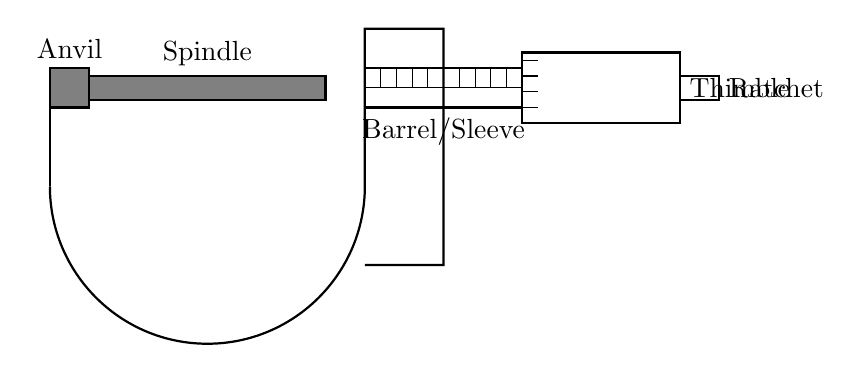
\begin{tikzpicture}
    % Frame
    \draw[thick] (0,0) arc (180:360:2cm) -- (4,0) -- (4,2) -- (5,2) -- (5,-1) -- (4,-1);
    \draw[thick] (0,0) -- (0,1);
    
    % Anvil
    \draw[thick, fill=gray] (0,1) rectangle (0.5,1.5);
    \node[above] at (0.25,1.5) {Anvil};
    
    % Spindle
    \draw[thick, fill=gray] (0.5,1.1) rectangle (3.5,1.4);
    \node[above] at (2,1.4) {Spindle};
    
    % Sleeve
    \draw[thick] (4,1) rectangle (6,1.5);
    \foreach \x in {4,4.2,...,6} \draw (\x,1.25) -- (\x,1.5);
    \draw (4,1.25) -- (6,1.25);
    \node[below] at (5,1) {Barrel/Sleeve};
    
    % Thimble
    \draw[thick] (6,0.8) rectangle (8,1.7);
    \foreach \y in {0.8,1.0,...,1.7} \draw (6,\y) -- (6.2,\y);
    \node[right] at (8,1.25) {Thimble};
    
    % Ratchet
    \draw[thick] (8,1.1) rectangle (8.5,1.4);
    \node[right] at (8.5,1.25) {Ratchet};
\end{tikzpicture}
\captionof{figure}{Micrometer Screw Gauge Components}
\end{center}

Common errors in micrometer screw gauge:
\begin{itemize}
    \item \textbf{Zero error}: When the measuring faces are in contact, the zero of thimble doesn't coincide with the datum line
    \begin{itemize}
        \item \textbf{Positive zero error}: When the zero mark on thimble is below the datum line
        \item \textbf{Negative zero error}: When the zero mark on thimble is above the datum line
    \end{itemize}
    \item \textbf{Backlash error}: Play between the screw and nut, causes different readings in forward and backward movement
    \item \textbf{Instrumental error}: Due to manufacturing defects or wear and tear
    \item \textbf{Parallax error}: When line of sight isn't perpendicular to scale reading
\end{itemize}

\textbf{Correction formula:} $\text{True reading} = \text{Observed reading} - \text{Zero error}$
\end{solutionbox}

\begin{mnemonicbox}
\mnemonic{ZBIP - Zero, Backlash, Instrument and Parallax errors make measurements trip}
\end{mnemonicbox}

\questionmarks{2(a)}{3}{Explain Coulomb's inverse square law.}

\begin{solutionbox}
Coulomb's inverse square law states that the electrostatic force between two point charges is:
\begin{itemize}
    \item Directly proportional to the product of the magnitudes of charges
    \item Inversely proportional to the square of the distance between them
    \item Acts along the line joining the two charges
\end{itemize}

\textbf{Mathematical expression:}
$$
F = k\frac{q_1q_2}{r^2}
$$

Where:
\begin{itemize}
    \item $F$ = Electrostatic force between charges
    \item $k$ = Coulomb's constant ($9 \times 10^9 \text{ N}\cdot\text{m}^2/\text{C}^2$)
    \item $q_1, q_2$ = Magnitudes of the two charges
    \item $r$ = Distance between the charges
\end{itemize}
\end{solutionbox}

\begin{mnemonicbox}
\mnemonic{PDSA - Product of charges Directly, Square of distance inversely, Along the line}
\end{mnemonicbox}

\questionmarks{2(b)}{4}{Explain electrical potential difference.}

\begin{solutionbox}
Electrical potential difference (voltage) is the work done per unit charge in moving a positive test charge between two points in an electric field.

\textbf{Mathematical expression:}
$$
V = \frac{W}{q}
$$

Where:
\begin{itemize}
    \item $V$ = Potential difference (volts)
    \item $W$ = Work done (joules)
    \item $q$ = Charge (coulombs)
\end{itemize}

\textbf{Key characteristics:}
\begin{itemize}
    \item Measured in volts (V)
    \item Scalar quantity (has magnitude only)
    \item Path independent (depends only on initial and final positions)
    \item Represents energy per unit charge
\end{itemize}
\end{solutionbox}

\begin{mnemonicbox}
\mnemonic{WPCS - Work Per Charge is what potential difference Says}
\end{mnemonicbox}

\questionmarks{2(c)}{7}{Explain equivalent capacitance of capacitors in series and in parallel combinations.}

\begin{solutionbox}
\textbf{Series Combination:}

\begin{center}
\begin{tikzpicture}
    \draw (0,0) to[C, l=$C_1$] (2,0) to[C, l=$C_2$] (4,0) to[C, l=$C_3$] (6,0);
    \draw (0,0) to[short, -o] (-0.5,0);
    \draw (6,0) to[short, -o] (6.5,0);
\end{tikzpicture}
\captionof{figure}{Capacitors in Series}
\end{center}

\begin{itemize}
    \item When capacitors are connected end-to-end
    \item Same charge on each capacitor: $Q = Q_1 = Q_2 = Q_3$
    \item Total potential difference: $V = V_1 + V_2 + V_3$
    \item Equivalent capacitance formula: $\frac{1}{C_{eq}} = \frac{1}{C_1} + \frac{1}{C_2} + \frac{1}{C_3} + ...$
    \item Equivalent capacitance is less than the smallest individual capacitance
\end{itemize}

\textbf{Parallel Combination:}

\begin{center}
\begin{tikzpicture}
    \draw (0,0) -- (1,0) -- (1,1.5) to[C, l=$C_1$] (4,1.5) -- (4,0) -- (5,0);
    \draw (1,0) to[C, l=$C_2$] (4,0);
    \draw (1,0) -- (1,-1.5) to[C, l=$C_3$] (4,-1.5) -- (4,0);
    \draw (0,0) to[short, -o] (-0.5,0);
    \draw (5,0) to[short, -o] (5.5,0);
\end{tikzpicture}
\captionof{figure}{Capacitors in Parallel}
\end{center}

\begin{itemize}
    \item When capacitors are connected between the same two points
    \item Same potential difference across each: $V = V_1 = V_2 = V_3$
    \item Total charge: $Q = Q_1 + Q_2 + Q_3$
    \item Equivalent capacitance formula: $C_{eq} = C_1 + C_2 + C_3 + ...$
    \item Equivalent capacitance is greater than the largest individual capacitance
\end{itemize}

\textbf{Comparison Table:}

\begin{center}
\captionof{table}{Series vs Parallel Capacitors}
\begin{tabulary}{\linewidth}{|L|L|L|}
\hline
\textbf{Parameter} & \textbf{Series} & \textbf{Parallel} \\ \hline
Charge & Same on all capacitors & Distributed as per capacitance \\ \hline
Voltage & Divided across capacitors & Same across all capacitors \\ \hline
Equivalent capacitance & $1/C_{eq} = 1/C_1 + 1/C_2 + ...$ & $C_{eq} = C_1 + C_2 + ...$ \\ \hline
Resulting capacitance & Smaller than any individual C & Larger than any individual C \\ \hline
\end{tabulary}
\end{center}
\end{solutionbox}

\begin{mnemonicbox}
\mnemonic{RAPS - Reciprocals Add in Parallel Sum}
\end{mnemonicbox}

\questionmarks{2(a) OR}{3}{Write characteristics of electrical lines.}

\begin{solutionbox}
\textbf{Characteristics of electric field lines:}
\begin{itemize}
    \item \textbf{Direction}: Always point from positive to negative charge
    \item \textbf{Nature}: Start from positive charge and end at negative charge
    \item \textbf{Continuity}: Never intersect each other
    \item \textbf{Density}: Closer lines indicate stronger electric field
    \item \textbf{Perpendicularity}: Always perpendicular to equipotential surfaces
    \item \textbf{Shape}: Straight lines for uniform fields, curved for non-uniform fields
    \item \textbf{Open/Closed}: Always open curves, unlike magnetic field lines
\end{itemize}
\end{solutionbox}

\begin{mnemonicbox}
\mnemonic{DNCPS - Direction, Never cross, Closeness shows strength, Perpendicular, Straight/curved}
\end{mnemonicbox}

\questionmarks{2(b) OR}{4}{Explain electric flux.}

\begin{solutionbox}
Electric flux is a measure of the electric field passing through a given area.

\textbf{Mathematical expression:}
$$
\Phi_E = E \cdot A \cdot \cos\theta
$$

Where:
\begin{itemize}
    \item $\Phi_E$ = Electric flux (N·m$^2$/C or V·m)
    \item $E$ = Electric field strength (N/C or V/m)
    \item $A$ = Area of the surface (m$^2$)
    \item $\theta$ = Angle between electric field and normal to the surface
\end{itemize}

\textbf{Key characteristics:}
\begin{itemize}
    \item Vector quantity
    \item SI unit is newton-meter-squared per coulomb (N·m$^2$/C) or volt-meter (V·m)
    \item Represents the number of field lines passing through a surface
    \item Maximum when field is perpendicular to surface ($\theta = 0^\circ$)
    \item Zero when field is parallel to surface ($\theta = 90^\circ$)
\end{itemize}
\end{solutionbox}

\begin{mnemonicbox}
\mnemonic{FACT - Flux = Area x Cos-theta x Field strength}
\end{mnemonicbox}

\questionmarks{2(c) OR}{7}{Explain capacitor and capacitance.}

\begin{solutionbox}
\textbf{Capacitor:}
A capacitor is an electrical component designed to store electric charge and energy in an electric field.

\textbf{Basic structure:}
\begin{center}
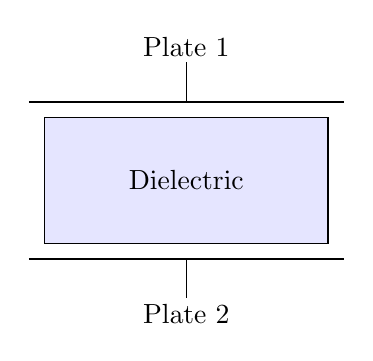
\begin{tikzpicture}
    % Plates
    \draw[thick] (0,2) -- (4,2);
    \draw[thick] (0,0) -- (4,0);
    
    % Dielectric
    \draw[fill=blue!10] (0.2,0.2) rectangle (3.8,1.8);
    \node at (2,1) {Dielectric};
    
    % Terminals
    \draw (2,2) -- (2,2.5);
    \draw (2,0) -- (2,-0.5);
    
    \node at (2,2.7) {Plate 1};
    \node at (2,-0.7) {Plate 2};
\end{tikzpicture}
\captionof{figure}{Parallel Plate Capacitor}
\end{center}

\textbf{Capacitance:}
The ability of a capacitor to store electric charge at a given potential difference.

\textbf{Mathematical expression:}
$$
C = \frac{Q}{V}
$$

Where:
\begin{itemize}
    \item $C$ = Capacitance (farads)
    \item $Q$ = Electric charge (coulombs)
    \item $V$ = Potential difference (volts)
\end{itemize}

\textbf{For a parallel plate capacitor:}
$$
C = \frac{\epsilon_0 \epsilon_r A}{d}
$$

Where:
\begin{itemize}
    \item $\epsilon_0$ = Permittivity of free space ($8.85 \times 10^{-12} \text{ F/m}$)
    \item $\epsilon_r$ = Relative permittivity of dielectric
    \item $A$ = Area of overlap between plates
    \item $d$ = Distance between plates
\end{itemize}

\textbf{Factors affecting capacitance:}
\begin{itemize}
    \item Increases with plate area
    \item Decreases with plate separation
    \item Increases with dielectric constant
\end{itemize}

\textbf{Applications of capacitors:}
\begin{itemize}
    \item Energy storage
    \item Filtering in power supplies
    \item Timing circuits
    \item Coupling and decoupling
    \item Power factor correction
\end{itemize}
\end{solutionbox}

\begin{mnemonicbox}
\mnemonic{QVAD - Quotient of charge and Voltage, affected by Area and Distance}
\end{mnemonicbox}

\questionmarks{3(a)}{3}{Define: (a) Heat radiation (b) Kilocalorie (c) Thermometer.}

\begin{solutionbox}
\begin{itemize}
    \item \textbf{Heat radiation}: The transfer of thermal energy in the form of electromagnetic waves without requiring a medium, occurring in vacuum or transparent media.
    \item \textbf{Kilocalorie}: A unit of heat energy equal to 1000 calories, where one calorie is the amount of heat required to raise the temperature of 1 gram of water by 1°C at standard conditions.
    \item \textbf{Thermometer}: An instrument used to measure temperature based on a physical property (like expansion of mercury) that changes with temperature.
\end{itemize}
\end{solutionbox}

\begin{mnemonicbox}
\mnemonic{RKT - Radiation needs no medium, Kilocalorie measures energy, Thermometer shows temperature}
\end{mnemonicbox}

\questionmarks{3(b)}{4}{Explain law of thermal conductivity.}

\begin{solutionbox}
The law of thermal conductivity (Fourier's law) states that the rate of heat transfer through a material is:
\begin{itemize}
    \item Directly proportional to the area of the section
    \item Directly proportional to the temperature gradient
    \item Dependent on the material's thermal conductivity
\end{itemize}

\textbf{Mathematical expression:}
$$
\frac{Q}{t} = -kA\frac{dT}{dx}
$$

Where:
\begin{itemize}
    \item $Q/t$ = Rate of heat transfer (J/s or W)
    \item $k$ = Thermal conductivity of material (W/m·K)
    \item $A$ = Cross-sectional area (m$^2$)
    \item $dT/dx$ = Temperature gradient (K/m)
    \item Negative sign indicates heat flows from higher to lower temperature
\end{itemize}
\end{solutionbox}

\begin{mnemonicbox}
\mnemonic{GAKT - Gradient And area with K gives heat Transfer}
\end{mnemonicbox}

\questionmarks{3(c)(1)}{3}{A person has a fever of 102°F. So how much would it be in Celsius and Kelvin?}

\begin{solutionbox}
\textbf{To convert from Fahrenheit to Celsius:}
$$
C = (F - 32) \times \frac{5}{9}
$$
$$
C = (102 - 32) \times \frac{5}{9}
$$
$$
C = 70 \times 0.555
$$
$$
C = 38.89^\circ C
$$

\textbf{To convert from Celsius to Kelvin:}
$$
K = C + 273.15
$$
$$
K = 38.89 + 273.15
$$
$$
K = 312.04 \text{ K}
$$

Therefore, $102^\circ F = 38.89^\circ C = 312.04 \text{ K}$
\end{solutionbox}

\begin{mnemonicbox}
\mnemonic{FSK - From Fahrenheit Subtract 32, multiply by 5/9, then add 273.15 for Kelvin}
\end{mnemonicbox}

\questionmarks{3(c)(2)}{4}{Explain Celsius and Fahrenheit scale.}

\begin{solutionbox}
\textbf{Comparison of Celsius and Fahrenheit Temperature Scales:}

\begin{center}
\captionof{table}{Celsius vs Fahrenheit}
\begin{tabulary}{\linewidth}{|L|L|L|}
\hline
\textbf{Parameter} & \textbf{Celsius Scale} & \textbf{Fahrenheit Scale} \\ \hline
Freezing point of water & 0°C & 32°F \\ \hline
Boiling point of water & 100°C & 212°F \\ \hline
Number of divisions & 100 divisions & 180 divisions \\ \hline
Developed by & Anders Celsius (1742) & Gabriel Fahrenheit (1724) \\ \hline
Used in & Most countries worldwide & Primarily USA and its territories \\ \hline
Relation & $C = (F - 32) \times 5/9$ & $F = (C \times 9/5) + 32$ \\ \hline
\end{tabulary}
\end{center}

\textbf{Diagram:}
\begin{center}
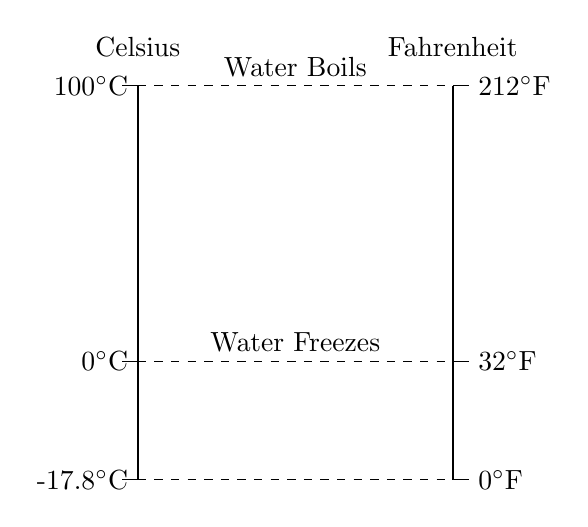
\begin{tikzpicture}
    % Celsius
    \draw[thick] (0,0) -- (0,5);
    \foreach \y/\t in {0/-17.8, 1.5/0, 5/100} \draw (-0.2,\y) -- (0,\y) node[left] {\t$^\circ$C};
    \node at (0, 5.5) {Celsius};
    
    % Fahrenheit
    \draw[thick] (4,0) -- (4,5);
    \foreach \y/\t in {0/0, 1.5/32, 5/212} \draw (4,\y) -- (4.2,\y) node[right] {\t$^\circ$F};
    \node at (4, 5.5) {Fahrenheit};
    
    % Connection lines
    \draw[dashed] (0,5) -- (4,5) node[midway, above] {Water Boils};
    \draw[dashed] (0,1.5) -- (4,1.5) node[midway, above] {Water Freezes};
    \draw[dashed] (0,0) -- (4,0);
\end{tikzpicture}
\captionof{figure}{Temperature Scales Comparison}
\end{center}
\end{solutionbox}

\begin{mnemonicbox}
\mnemonic{FBIC - Fahrenheit has Bigger numbers, Interval of 180, Conversion needs 5/9 or 9/5}
\end{mnemonicbox}

\questionmarks{3(a) OR}{3}{Write definition, formula and unit of Heat capacity.}

\begin{solutionbox}
\textbf{Definition:} Heat capacity is the amount of heat energy required to raise the temperature of an object by one degree (Celsius or Kelvin).

\textbf{Formula:}
$$
C = \frac{Q}{\Delta T}
$$

Where:
\begin{itemize}
    \item $C$ = Heat capacity (J/K or J/$^\circ$C)
    \item $Q$ = Heat energy supplied (joules)
    \item $\Delta T$ = Change in temperature (K or $^\circ$C)
\end{itemize}

\textbf{Units:} Joules per kelvin (J/K) or joules per degree Celsius (J/$^\circ$C)
\end{solutionbox}

\begin{mnemonicbox}
\mnemonic{QTC - Quotient of heat and Temperature Change gives heat capacity}
\end{mnemonicbox}

\questionmarks{3(b) OR}{4}{Explain Modes of Heat Transfer}

\begin{solutionbox}
\textbf{Three modes of heat transfer:}

\begin{center}
\captionof{table}{Modes of Heat Transfer}
\begin{tabulary}{\linewidth}{|L|L|L|L|}
\hline
\textbf{Mode} & \textbf{Definition} & \textbf{Examples} & \textbf{Medium Required} \\ \hline
\textbf{Conduction} & Transfer of heat through direct molecular collision without bulk motion of matter & Heat through metal rod, cooking pan & Yes (solid preferred) \\ \hline
\textbf{Convection} & Transfer of heat by movement of heated particles from one region to another & Boiling water, room heater, sea breeze & Yes (fluid - liquid or gas) \\ \hline
\textbf{Radiation} & Transfer of heat via electromagnetic waves without requiring medium & Solar radiation, microwave heating, infrared heaters & No (works in vacuum) \\ \hline
\end{tabulary}
\end{center}
\end{solutionbox}

\begin{mnemonicbox}
\mnemonic{CoCRa - Conduction needs Contact, Convection needs Currents, Radiation needs no medium}
\end{mnemonicbox}

\questionmarks{3(c) OR}{7}{Explain bimetallic thermometer.}

\begin{solutionbox}
\textbf{Diagram:}
\begin{center}
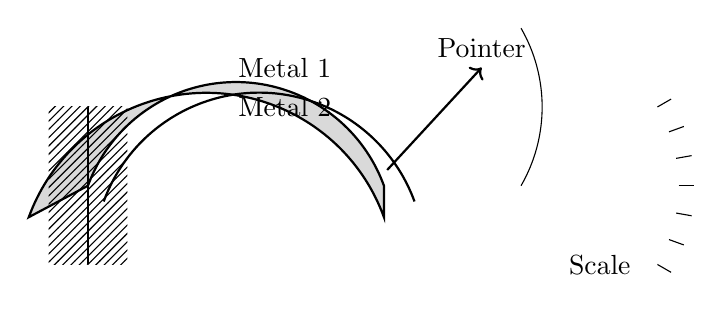
\begin{tikzpicture}
    % Strip
    \draw[thick, fill=gray!30] (0,0) arc (160:20:2) -- ++(0,-0.4) arc (20:160:2.4) -- cycle;
    \draw[thick] (0.2,-0.2) arc (160:20:2.1); % Dividing line
    \node at (2.5,1.5) {Metal 1};
    \node at (2.5,1.0) {Metal 2};
    
    % Pointer
    \draw[thick, ->] (3.8,0.2) -- (5,1.5);
    \node[above] at (5,1.5) {Pointer};
    
    % Scale
    \draw (5.5,0) arc (-30:30:2);
    \foreach \a in {-30,-20,...,30} \draw (5.5,0) ++(\a:2) -- ++(\a:0.2);
    \node at (6.5,-1) {Scale};
    
    % Fixed end
    \fill[pattern=north east lines] (-0.5,-1) rectangle (0.5,1);
    \draw (0,-1) -- (0,1);
\end{tikzpicture}
\captionof{figure}{Bimetallic Strip Thermometer}
\end{center}

\textbf{Working principle:}
\begin{itemize}
    \item Based on differential thermal expansion of two different metals
    \item Two metal strips with different coefficients of thermal expansion are bonded together
    \item When heated, one metal expands more than the other
    \item This uneven expansion causes the strip to bend toward the metal with lower expansion
    \item The amount of bending is proportional to temperature change
    \item A pointer attached to the strip indicates temperature on a calibrated scale
\end{itemize}

\textbf{Advantages:}
\begin{itemize}
    \item Simple, robust construction
    \item No liquid or gas required
    \item Wide temperature range
    \item Resistant to mechanical shocks
    \item Can be used to make thermostats
\end{itemize}

\textbf{Applications:} Thermostats, automobile cooling systems, oven controls, circuit breakers.
\end{solutionbox}

\begin{mnemonicbox}
\mnemonic{BENDS - Bimetallic strips Expand, Not equally, Different metals, Show temperature}
\end{mnemonicbox}

\questionmarks{4(a)}{3}{Define: (a) Frequency (b) Infrasonic waves (c) Echo.}

\begin{solutionbox}
\begin{itemize}
    \item \textbf{Frequency}: The number of complete oscillations or cycles per unit time, measured in hertz (Hz).
    \item \textbf{Infrasonic waves}: Sound waves with frequencies below the lower limit of human hearing (below 20 Hz) that cannot be heard by humans but may be detected by other animals.
    \item \textbf{Echo}: A sound that is reflected back to the listener with sufficient time delay to be heard as a distinct repetition of the original sound.
\end{itemize}
\end{solutionbox}

\begin{mnemonicbox}
\mnemonic{FIE - Frequency counts cycles, Infrasonic is below hearing, Echo comes back after reflection}
\end{mnemonicbox}

\questionmarks{4(b)}{4}{Give distinction between Longitudinal and Transverse waves.}

\begin{solutionbox}
\textbf{Comparison between Longitudinal and Transverse Waves:}

\begin{center}
\captionof{table}{Longitudinal vs Transverse Waves}
\begin{tabulary}{\linewidth}{|L|L|L|}
\hline
\textbf{Parameter} & \textbf{Longitudinal Waves} & \textbf{Transverse Waves} \\ \hline
Direction of particle motion & Parallel to wave propagation & Perpendicular to wave propagation \\ \hline
Example & Sound waves, P-waves & Light waves, ripples on water \\ \hline
Medium requirement & Solids, liquids and gases & Solids and surfaces of liquids (not gases) \\ \hline
Components & Compressions and rarefactions & Crests and troughs \\ \hline
Polarization & Cannot be polarized & Can be polarized \\ \hline
Visualization & Spring/Slinky & Rope moving up and down \\ \hline
\end{tabulary}
\end{center}

\textbf{Diagram:}
\begin{center}
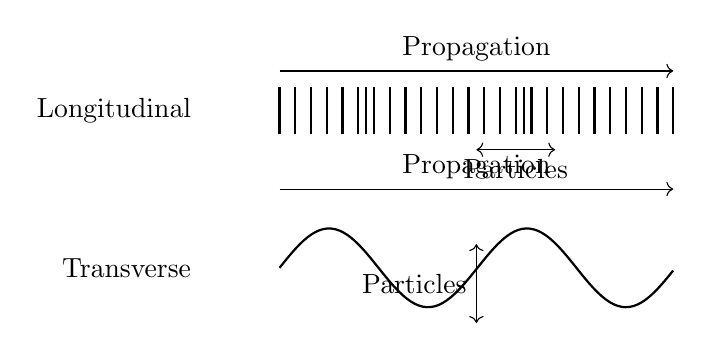
\begin{tikzpicture}
    % Longitudinal
    \node[left] at (-1,1.5) {Longitudinal};
    \foreach \x in {0,0.2,...,5} {
        \draw[thick] (\x,1.2) -- (\x,1.8);
    }
    % Compressions
    \foreach \x in {1,1.1,1.2, 3,3.1,3.2} {
        \draw[thick] (\x,1.2) -- (\x,1.8);
    }
    \draw[->] (0,2) -- (5,2) node[midway, above] {Propagation};
    \draw[<->] (2.5,1) -- (3.5,1) node[midway, below] {Particles};
    
    % Transverse
    \node[left] at (-1,-0.5) {Transverse};
    \draw[thick, domain=0:5, samples=100] plot (\x, {sin(\x r * 2.5) * 0.5 - 0.5});
    \draw[->] (0,0.5) -- (5,0.5) node[midway, above] {Propagation};
    \draw[<->] (2.5,-1.2) -- (2.5,-0.2) node[midway, left] {Particles};
\end{tikzpicture}
\captionof{figure}{Wave Types}
\end{center}
\end{solutionbox}

\begin{mnemonicbox}
\mnemonic{PPCP - Particles move Parallel in Longitudinal, Perpendicular in Transverse, Compressions vs Crests, Polarization only in Transverse}
\end{mnemonicbox}

\questionmarks{4(c)(1)}{4}{Give three properties and uses of ultrasonic waves.}

\begin{solutionbox}
\textbf{Properties of ultrasonic waves:}
\begin{itemize}
    \item Frequency ranges above 20,000 Hz (beyond human hearing)
    \item Short wavelengths allow detection of small objects
    \item High directivity compared to audible sound
    \item High penetration in certain media
    \item Less diffraction around obstacles
    \item Cause cavitation in liquids
\end{itemize}

\textbf{Uses of ultrasonic waves:}
\begin{center}
\captionof{table}{Uses of Ultrasonic Waves}
\begin{tabulary}{\linewidth}{|L|L|}
\hline
\textbf{Field} & \textbf{Applications} \\ \hline
\textbf{Medical} & Sonography, kidney stone destruction, physiotherapy \\ \hline
\textbf{Industrial} & Non-destructive testing, cleaning, welding, drilling \\ \hline
\textbf{Navigation} & SONAR, distance measurement, obstacle detection \\ \hline
\textbf{Other} & Dog whistles, pest control, echolocation \\ \hline
\end{tabulary}
\end{center}
\end{solutionbox}

\begin{mnemonicbox}
\mnemonic{FWD-MNO - Frequency high, Wavelength short, Direction focused; Medical imaging, NDT testing, Ocean mapping}
\end{mnemonicbox}

\questionmarks{4(c)(2)}{3}{Derive relation between velocity, wavelength and frequency.}

\begin{solutionbox}
\textbf{Derivation:}
Consider a wave traveling with:
\begin{itemize}
    \item Wavelength ($\lambda$): Distance between consecutive similar points
    \item Frequency ($f$): Number of waves passing a point per second
    \item Time period ($T$): Time to complete one cycle
\end{itemize}

During one time period ($T$), the wave travels a distance equal to one wavelength ($\lambda$).
$$
\text{Velocity} = \frac{\text{Distance}}{\text{Time}} = \frac{\lambda}{T}
$$
Since frequency $f = 1/T$, we can write:
$$
v = \lambda \times f
$$
Where $v$ is velocity (m/s), $\lambda$ is wavelength (m), and $f$ is frequency (Hz).

\textbf{Diagram:}
\begin{center}
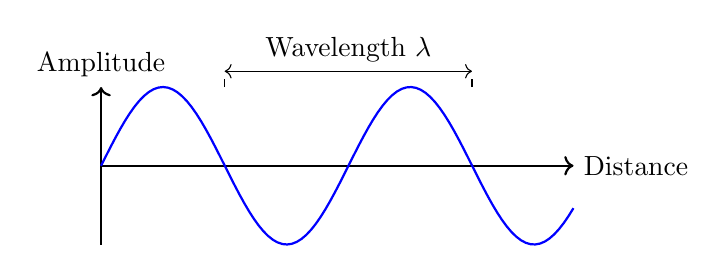
\begin{tikzpicture}
    \draw[thick, ->] (0,0) -- (6,0) node[right] {Distance};
    \draw[thick, ->] (0,-1) -- (0,1) node[above] {Amplitude};
    \draw[thick, blue, domain=0:6, samples=100] plot (\x, {sin(\x r * 2)});
    
    \draw[<->] (1.57,1.2) -- (4.71,1.2) node[midway, above] {Wavelength $\lambda$};
    \draw[dashed] (1.57,1) -- (1.57,1.2);
    \draw[dashed] (4.71,1) -- (4.71,1.2);
\end{tikzpicture}
\captionof{figure}{Wavelength Visualization}
\end{center}
\end{solutionbox}

\begin{mnemonicbox}
\mnemonic{VLF - Velocity equals Lambda times Frequency}
\end{mnemonicbox}

\questionmarks{4(a) OR}{3}{Explain Sabine's formula for reverberation time.}

\begin{solutionbox}
Sabine's formula calculates the reverberation time in an enclosed space:

\textbf{Formula:}
$$
RT_{60} = \frac{0.161 \times V}{A}
$$

Where:
\begin{itemize}
    \item $RT_{60}$ = Reverberation time (seconds) for sound to decay by 60 dB
    \item $V$ = Volume of the room (m$^3$)
    \item $A$ = Total sound absorption (m$^2$ sabins)
\end{itemize}

\textbf{Total absorption ($A$)} is calculated as:
$$
A = \sum \alpha_i S_i = \alpha_1 S_1 + \alpha_2 S_2 + ...
$$
Where $\alpha_i$ is absorption coefficient and $S_i$ is surface area.

\end{solutionbox}

\begin{mnemonicbox}
\mnemonic{VAS - Volume And Surface absorption determine reverberation time}
\end{mnemonicbox}

\questionmarks{4(b) OR}{4}{What is diffraction of light? Explain its types with diagram.}

\begin{solutionbox}
\textbf{Definition:} Diffraction is the bending of light waves around obstacles or through openings, showing the wave nature of light.

\textbf{Types of diffraction:}

1. \textbf{Fresnel Diffraction}: Source or screen at finite distance. Spherical wavefronts. Complex pattern.

\begin{center}
\begin{tikzpicture}
    \node[circle, fill, inner sep=1.5pt] (S) at (0,0) {}; \node[left] at (S) {Source};
    \draw[thick] (2,-1) -- (2,1); \draw[white, thick] (2,-0.2) -- (2,0.2); % Opening
    \draw[thick] (4,-1.5) -- (4,1.5); \node[right] at (4,0) {Screen};
    
    \draw[->] (S) -- (2,0.2);
    \draw[->] (S) -- (2,-0.2);
\end{tikzpicture}
\captionof{figure}{Fresnel Diffraction}
\end{center}

2. \textbf{Fraunhofer Diffraction}: Source and screen at infinite distance. Plane wavefronts. Simple pattern.

\begin{center}
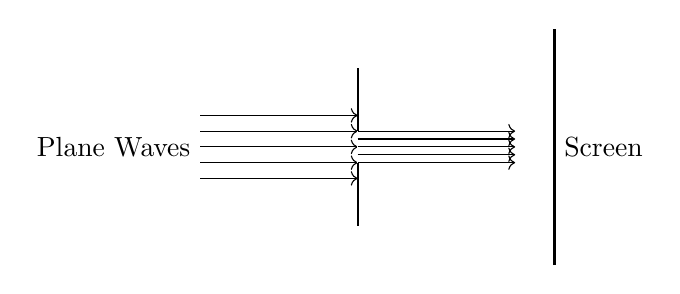
\begin{tikzpicture}
    \foreach \y in {-0.4,-0.2,0,0.2,0.4} \draw[->] (0,\y) -- (2,\y);
    \node[left] at (0,0) {Plane Waves};
    
    \draw[thick] (2,-1) -- (2,1); \draw[white, thick] (2,-0.2) -- (2,0.2); % Opening
    
    \foreach \y in {-0.4,-0.2,0,0.2,0.4} \draw[->] (2,\y*0.5) -- (4,\y*0.5); % Diffracted? Actually focusing
    
    \draw[thick] (4.5,-1.5) -- (4.5,1.5); \node[right] at (4.5,0) {Screen};
\end{tikzpicture}
\captionof{figure}{Fraunhofer Diffraction}
\end{center}
\end{solutionbox}

\begin{mnemonicbox}
\mnemonic{FPSS - Fresnel has Finite distances, Spherical waves; Fraunhofer has Source at infinity, Straight (plane) waves}
\end{mnemonicbox}

\questionmarks{4(c)(1) OR}{3}{Find the wavelength of a radio wave if the frequency is 480 Hz and the speed of sound is 330 m/s.}

\begin{solutionbox}
\textbf{Given:}
\begin{itemize}
    \item Frequency ($f$) = 480 Hz
    \item Speed ($v$) = 330 m/s
\end{itemize}

\textbf{To find:} Wavelength ($\lambda$)

\textbf{Formula:} $v = \lambda \times f \Rightarrow \lambda = v/f$

\textbf{Calculation:}
$$
\lambda = \frac{330}{480} = 0.6875 \text{ m}
$$

Therefore, the wavelength is 0.6875 m or 68.75 cm.
\end{solutionbox}

\begin{mnemonicbox}
\mnemonic{WFV - Wavelength equals Velocity divided by Frequency}
\end{mnemonicbox}

\questionmarks{4(c)(2) OR}{4}{Give properties of sound waves}

\begin{solutionbox}
\textbf{Properties of sound waves:}

\begin{center}
\captionof{table}{Sound Wave Properties}
\begin{tabulary}{\linewidth}{|L|L|}
\hline
\textbf{Property} & \textbf{Description} \\ \hline
Wave nature & Mechanical, longitudinal wave requiring a medium \\ \hline
Frequency range & Audible range: 20 Hz to 20,000 Hz \\ \hline
Speed & ~343 m/s in air; fastest in solids \\ \hline
Reflection & Bounces off surfaces (echoes) \\ \hline
Refraction & Changes direction between media \\ \hline
Diffraction & Bends around obstacles \\ \hline
Interference & Constructive or destructive superposition \\ \hline
Resonance & Amplification at natural frequencies \\ \hline
\end{tabulary}
\end{center}
\end{solutionbox}

\begin{mnemonicbox}
\mnemonic{WARDS-FIR - Wave needs medium, Audible range limited, Reflected, Diffracted, Speed varies, Frequency determines pitch, Intensity determines loudness, Resonates at natural frequencies}
\end{mnemonicbox}

\questionmarks{5(a)}{3}{State the meaning and properties of Laser.}

\begin{solutionbox}
\textbf{LASER}: Light Amplification by Stimulated Emission of Radiation

\textbf{Properties of laser light:}
\begin{itemize}
    \item \textbf{Monochromatic}: Single wavelength
    \item \textbf{Coherent}: Waves are in phase
    \item \textbf{Directional}: Travels in straight line, low divergence
    \item \textbf{Intense}: High energy concentration
    \item \textbf{Collimated}: Rays are parallel
\end{itemize}
\end{solutionbox}

\begin{mnemonicbox}
\mnemonic{MCCDI - Monochromatic and Coherent, Collimated, Directional, Intense}
\end{mnemonicbox}

\questionmarks{5(b)}{4}{Give information about optical fiber.}

\begin{solutionbox}
\textbf{Optical Fiber}: Flexible, transparent fiber giving light signals through total internal reflection.

\textbf{Structure:}
\begin{center}
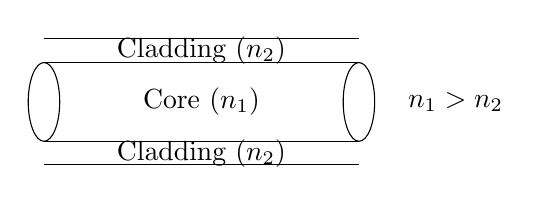
\begin{tikzpicture}
    \draw[fill=white] (0,0) ellipse (0.2 and 0.5); % Core end
    \draw (0,0.5) -- (4,0.5);
    \draw (0,-0.5) -- (4,-0.5);
    \draw (4,0) ellipse (0.2 and 0.5);
    \node at (2,0) {Core ($n_1$)};
    
    \draw (0,0.8) -- (4,0.8);
    \draw (0,-0.8) -- (4,-0.8);
    \node at (2,0.65) {Cladding ($n_2$)};
    \node at (2,-0.65) {Cladding ($n_2$)};
    
    \node[right] at (4.5,0) {$n_1 > n_2$};
\end{tikzpicture}
\captionof{figure}{Optical Fiber Structure}
\end{center}

\textbf{Components:}
\begin{itemize}
    \item \textbf{Core}: Central region (high refractive index)
    \item \textbf{Cladding}: Outer optical material (lower refractive index)
    \item \textbf{Buffer coating}: Protective covering
\end{itemize}

\textbf{Types:} Single-mode (small core), Multi-mode (large core).
\end{solutionbox}

\begin{mnemonicbox}
\mnemonic{CCTLT - Core Carries light, Cladding keeps it in, Total internal reflection, Low loss transmission}
\end{mnemonicbox}

\questionmarks{5(c)(1)}{7}{Explain Snell's law.}

\begin{solutionbox}
\textbf{Definition:} Snell's law states that the ratio of the sine of the angle of incidence to the sine of the angle of refraction is constant.

\textbf{Formula:} $n_1 \sin(\theta_1) = n_2 \sin(\theta_2)$

\textbf{Diagram:}
\begin{center}
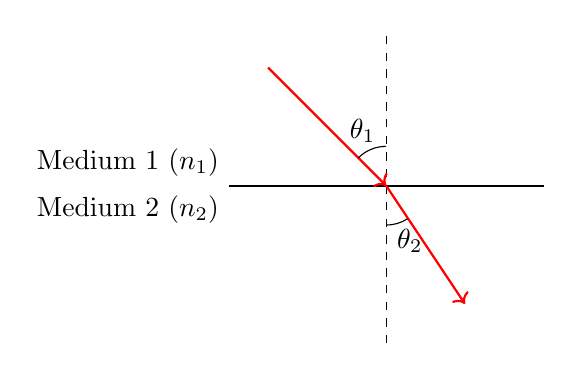
\begin{tikzpicture}
    % Boundary
    \draw[thick] (-2,0) -- (2,0);
    \node[above left] at (-2,0) {Medium 1 ($n_1$)};
    \node[below left] at (-2,0) {Medium 2 ($n_2$)};
    
    % Normal
    \draw[dashed] (0,-2) -- (0,2);
    
    % Rays
    \draw[thick, red, ->] (-1.5,1.5) -- (0,0);
    \draw[thick, red, ->] (0,0) -- (1,-1.5);
    
    % Angles
    \draw (0,0.5) arc (90:135:0.5);
    \node at (-0.3,0.7) {$\theta_1$};
    
    \draw (0,-0.5) arc (270:303:0.5);
    \node at (0.3,-0.7) {$\theta_2$};
\end{tikzpicture}
\captionof{figure}{Refraction (Snell's Law)}
\end{center}
\end{solutionbox}

\begin{mnemonicbox}
\mnemonic{SINS - Sine of incidence over sine of refraction equals N1 over N2}
\end{mnemonicbox}

\questionmarks{5(c)(2)}{0}{Explain the Acceptance angle.}

\begin{solutionbox}
\textbf{Acceptance angle} is the maximum angle at which light can enter an optical fiber and still experience total internal reflection.

\textbf{Formula:} $\theta_a = \sin^{-1}(NA)$ where $NA = \sqrt{n_1^2 - n_2^2}$

\textbf{Diagram:}
\begin{center}
\begin{tikzpicture}
    % Fiber face
    \draw[thick] (2,-1) -- (2,1);
    \draw[thick] (2,0.5) -- (6,0.5);
    \draw[thick] (2,-0.5) -- (6,-0.5);
    
    % Cone
    \draw[dashed] (0,0) -- (2,0.5);
    \draw[dashed] (0,0) -- (2,-0.5);
    \draw[->] (1,0) arc (0:14:1);
    \node at (1.5,0.1) {$\theta_a$};
    
    % Axis
    \draw[dotted] (-1,0) -- (6,0);
\end{tikzpicture}
\captionof{figure}{Acceptance Cone}
\end{center}
\end{solutionbox}

\begin{mnemonicbox}
\mnemonic{CAP - Core and cladding indices Affect the acceptance angle}
\end{mnemonicbox}

\questionmarks{5(a) OR}{3}{Write the uses of Laser.}

\begin{solutionbox}
\textbf{Uses of Laser:}
\begin{center}
\captionof{table}{Laser Applications}
\begin{tabulary}{\linewidth}{|L|L|}
\hline
\textbf{Field} & \textbf{Applications} \\ \hline
Medical & Surgery, eye treatment, cancer therapy \\ \hline
Industrial & Cutting, welding, 3D printing \\ \hline
Communications & Fiber optics \\ \hline
Scientific & Spectroscopy, holography \\ \hline
Consumer & Barcode scanners, printers \\ \hline
Military & Range finding, weapons \\ \hline
\end{tabulary}
\end{center}
\end{solutionbox}

\begin{mnemonicbox}
\mnemonic{MICSM - Medical, Industrial, Communication, Scientific, Military}
\end{mnemonicbox}

\questionmarks{5(b) OR}{4}{Write a short note on total internal reflection of light.}

\begin{solutionbox}
\textbf{Total Internal Reflection (TIR)} occurs when light traveling in a denser medium hits the boundary with a less dense medium at an angle greater than the critical angle.

\textbf{Conditions:}
\begin{itemize}
    \item Light must travel from denser to less dense medium ($n_1 > n_2$)
    \item Angle of incidence > Critical angle ($\theta_i > \theta_c$)
\end{itemize}

\textbf{Critical angle formula:} $\theta_c = \sin^{-1}(n_2/n_1)$

\textbf{Diagram:}
\begin{center}
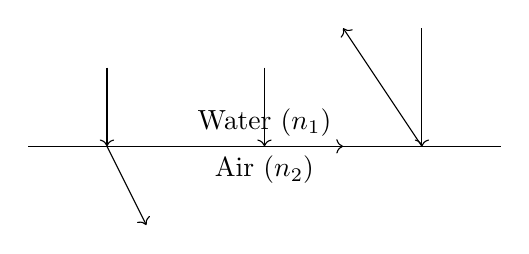
\begin{tikzpicture}
    \draw (-3,0) -- (3,0);
    \node[below] at (0,0) {Air ($n_2$)};
    \node[above] at (0,0) {Water ($n_1$)};
    
    % Case 1: Refraction
    \draw[->] (-2,1) -- (-2,0);
    \draw[->] (-2,0) -- (-1.5,-1);
    
    % Case 2: Critical
    \draw[->] (0,1) -- (0,0);
    \draw[->] (0,0) -- (1,0); 
    
    % Case 3: TIR
    \draw[->] (2,1.5) -- (2,0);
    \draw[->] (2,0) -- (1,1.5);
\end{tikzpicture}
\captionof{figure}{Total Internal Reflection}
\end{center}
\end{solutionbox}

\begin{mnemonicbox}
\mnemonic{CANDO - Critical Angle, N1 Denser, Only when angle > Critical}
\end{mnemonicbox}

\questionmarks{5(c)(1) OR}{3}{If the speed of light in water is $2.25 \times 10^8$ m/s and in air is $3 \times 10^8$ m/s, find refractive index of water.}

\begin{solutionbox}
\textbf{Given:}
\begin{itemize}
    \item $v_w = 2.25 \times 10^8$ m/s
    \item $v_a = 3 \times 10^8$ m/s
\end{itemize}

\textbf{Formula:} $n = c/v \Rightarrow n_w = v_a/v_w$

\textbf{Calculation:}
$$
n_w = \frac{3 \times 10^8}{2.25 \times 10^8} = \frac{3}{2.25} = 1.33
$$

Therefore, the refractive index of water is 1.33.
\end{solutionbox}

\begin{mnemonicbox}
\mnemonic{SVN - Speed in Vacuum divided by Speed in medium gives refractive iNdex}
\end{mnemonicbox}

\questionmarks{5(c)(2) OR}{4}{Write a note on step index fiber.}

\begin{solutionbox}
\textbf{Step Index Fiber:}
Optical fiber where refractive index changes abruptly between core and cladding.

\textbf{Characteristics:}
\begin{itemize}
    \item Abrupt change in index
    \item Single-mode or Multi-mode
    \item Simpler construction
    \item Higher modal dispersion in multi-mode
\end{itemize}

\textbf{Diagram:}
\begin{center}
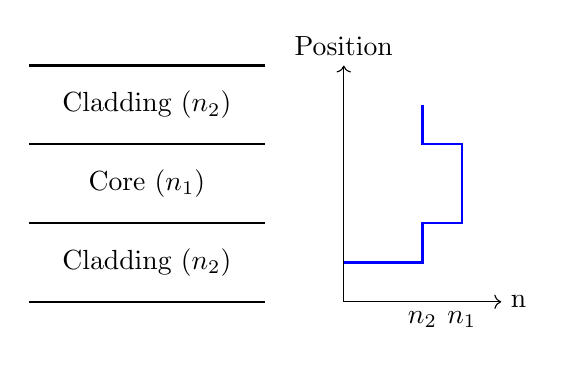
\begin{tikzpicture}
    % Fiber profile
    \draw[thick] (0,0) -- (3,0);
    \draw[thick] (0,1) -- (3,1);
    \draw[thick] (0,2) -- (3,2);
    \draw[thick] (0,3) -- (3,3);
    
    \node at (1.5,0.5) {Cladding ($n_2$)};
    \node at (1.5,1.5) {Core ($n_1$)};
    \node at (1.5,2.5) {Cladding ($n_2$)};
    
    % RI Profile
    \draw[->] (4,0) -- (6,0) node[right] {n};
    \draw[->] (4,0) -- (4,3) node[above] {Position};
    
    \draw[thick, blue] (4,0.5) -- (5,0.5) -- (5,1) -- (5.5,1) -- (5.5,2) -- (5,2) -- (5,2.5);
    \node[below] at (5,0) {$n_2$};
    \node[below] at (5.5,0) {$n_1$};
\end{tikzpicture}
\captionof{figure}{Step Index Fiber Profile}
\end{center}
\end{solutionbox}

\begin{mnemonicbox}
\mnemonic{SACS - Step change, Abrupt profile, Core guides, Simple}
\end{mnemonicbox}

\end{document}
